% arXiv paper template
\documentclass[11pt,letterpaper]{article}
\usepackage[utf8]{inputenc}
\usepackage[T1]{fontenc}
\usepackage{amsmath,amsfonts,amssymb}
\usepackage{graphicx}
\usepackage{tikz}
\usetikzlibrary{arrows.meta, positioning, shapes.geometric, shapes.misc}
\usepackage{hyperref}
\usepackage{algorithm}
\usepackage{algorithmic}
\usepackage{listings}
\usepackage{xcolor}
\usepackage{booktabs}

% Page geometry
\usepackage[margin=1in]{geometry}

% Code listing style
\lstset{
  basicstyle=\ttfamily\small,
  breaklines=true,
  frame=single,
  numbers=left
}

\title{Deterministic Runtime Enforcement for AI Governance}

\author{
  James Benton \\
  ExecLayer Inc., Wilmington, Delaware, United States \\
  \texttt{press@execlayer.io}
}

\date{}

\begin{document}

\maketitle

\begin{abstract}
Autonomous AI systems increasingly execute operational actions across critical domains including healthcare, finance, and infrastructure. Current governance approaches rely on risk classification taxonomies, organizational policies, and retrospective audit mechanisms that lack verifiable enforcement at the execution boundary. This creates a governance verification gap where compliance intent cannot be reliably translated into operational constraint. Process-based governance models assume organizational discipline but provide no architectural guarantee that AI systems operate within authorized parameters.

This paper introduces a deterministic runtime enforcement model that positions mandatory authorization checkpoints at the operational boundary where AI-generated intent transitions to system execution. The model employs an intermediate schema representation termed a Blueprint that encodes operations, authority requirements, risk classifications, and execution constraints in declarative form. Enforcement occurs through cryptographic Trust Artifacts that provide verifiable evidence of pre-execution authorization decisions. The architecture enables fail-closed operation where unauthorized actions are prevented rather than detected retrospectively.

The paper formalizes the enforcement model, demonstrates how it addresses structural limitations in audit-based governance, and analyzes formal properties including determinism, non-bypassability under stated assumptions, and audit completeness. We describe an implementation validating feasibility. The approach is compatible with regulatory frameworks requiring verifiable AI system compliance including ISO 42001, NIST AI RMF, and EU AI Act high-risk system requirements.
\end{abstract}

\noindent\textbf{Keywords:} AI governance; runtime enforcement; cryptographic authorization; deterministic execution; compliance verification

\section{Introduction}

The deployment of autonomous AI systems has transitioned from experimental settings to operational infrastructure managing real-world processes. Large language models and multi-agent systems now possess capability to invoke application programming interfaces, modify databases, initiate financial transactions, control physical systems, and orchestrate complex workflows across organizational boundaries. This expansion introduces fundamental governance challenges that conventional policy frameworks cannot adequately address.

Traditional software systems execute deterministically from explicitly programmed code paths where authorization decisions are embedded in access control logic. Execution authority is verifiable through code review and configuration inspection. AI systems fundamentally differ: operational decisions emerge from probabilistic inference over learned patterns rather than deterministic execution of predefined logic. When an AI agent decides to execute a database modification or external API invocation, that decision derives from model weights and prompt context rather than explicit authorization grants.

This architectural difference creates what we term the \textbf{governance verification gap}: the inability to verify that an AI system's actual operational behavior aligns with documented governance commitments at execution time. Organizations can assert compliance with frameworks such as ISO 42001 or the EU AI Act through policy documentation and periodic audits, yet lack technical mechanisms to ensure those policies constrain execution in practice.

\subsection{The Risk Classification Limitation}

Contemporary AI governance frameworks employ risk-based taxonomies where systems are classified by potential harm severity, with oversight requirements scaled accordingly. The EU AI Act defines four risk tiers (unacceptable, high, limited, minimal) with corresponding regulatory obligations. NIST's AI Risk Management Framework prescribes risk assessment driving control selection. ISO 42001 specifies risk-based approaches to AI management systems.

While conceptually sound, risk classification exhibits structural limitations when applied to AI systems:

\textbf{Classification Instability}: An AI system's risk level depends on deployment context and operational parameters rather than inherent system properties. A customer service agent classified as ``limited risk'' becomes high-risk when granted database write authority or financial transaction capability. Static classification cannot capture dynamic operational risk.

\textbf{Self-Assessment Failure}: Organizations classify their own systems with obvious incentive misalignment. External auditors reviewing classifications lack visibility into actual operational behavior and must rely on organizational representations.

\textbf{Control Ambiguity}: Risk tiers specify required controls (logging, human oversight, transparency) but not technical enforcement mechanisms. Organizations can document control implementation while retaining technical capability to bypass controls during execution.

\textbf{Temporal Drift}: Authorization decisions made at deployment time become stale as operational contexts evolve, yet no architectural mechanism ensures runtime reconciliation against current policies.

\subsection{Audit Theater and Verification Limits}

Conventional compliance audits examine documentation of governance procedures, evidence of training completion, samples of system outputs, and incident response records. What audits cannot examine is whether documented controls actually prevent non-compliant operations from executing. This creates \textbf{audit theater} where organizations demonstrate governance process existence without proving operational constraint.

The limitation intensifies for AI systems because traditional audit evidence becomes uninformative. Code review provides no insight into behavior emerging from model weights. Training data analysis reveals little about responses to novel production inputs. Configuration inspection cannot predict outputs from probabilistic inference.

Post-execution audit trails detect violations retrospectively after potential harm occurs. Audit logs are generated by the systems being audited, enabling selective disclosure or manipulation. Cross-system workflows create attribution challenges where no single component possesses visibility into complete authorization chains. Sophisticated attackers manipulate logs to conceal unauthorized actions.

\subsection{The Execution Boundary Problem}

Authorization enforcement can occur at three possible layers:

\textbf{Intent Generation Layer}: Preventing AI models from generating non-compliant intent through training constraints, fine-tuning, or prompt engineering. This approach is probabilistic---models may generate harmful intent despite training safeguards. Enforcement reliability is insufficient for critical applications.

\textbf{Execution Layer}: Validating that operations about to execute possess required authorization according to applicable policies, regardless of intent source. This approach is deterministic---unauthorized operations are blocked with cryptographic certainty prior to execution.

\textbf{Outcome Assessment Layer}: Evaluating whether executed operations satisfied governance requirements by analyzing outcomes. This approach is retrospective---harm may have occurred before non-compliance detection.

Only execution layer enforcement provides both deterministic prevention and pre-execution timeliness.

\subsection{Contribution Summary}

This paper makes the following contributions:

\begin{enumerate}
\item \textbf{Formalization of execution-bound governance} as architectural layer positioned between intent generation and operational execution, with formal definition of enforcement properties.

\item \textbf{Deterministic authorization checkpoint model} employing fail-closed semantics where execution proceeds only upon explicit authorization following successful policy validation.

\item \textbf{Blueprint intermediate schema} providing declarative representation of operational intent that explicitly encodes authority requirements, risk classifications, and execution constraints in machine-verifiable form.

\item \textbf{Cryptographic trust artifact structure} enabling portable verification of authorization decisions through tamper-evident records with verifiable authority lineage.

\item \textbf{Analysis of enforcement properties} including determinism under operational assumptions, non-bypassability conditions, pre-execution constraint validation, audit completeness, and lineage integrity with explicit limitation acknowledgment.
\end{enumerate}

The model is compatible with risk-based governance frameworks including ISO 42001, NIST AI RMF, and the EU AI Act.

The remainder of this paper proceeds as follows. Section~\ref{sec:background} reviews related work in AI governance frameworks and access control architectures. Section~\ref{sec:threat} formalizes the threat model. Section~\ref{sec:model} presents the enforcement model with Blueprint schema, validation logic, and trust artifact structure. Section~\ref{sec:properties} analyzes formal properties. Section~\ref{sec:comparison} provides comparative analysis against process-based approaches. Section~\ref{sec:implementation} discusses implementation considerations. Section~\ref{sec:limitations} acknowledges limitations. Section~\ref{sec:conclusion} concludes.

\section{Background and Related Work}
\label{sec:background}

\subsection{AI Governance Frameworks}

Several regulatory and standards frameworks address AI system governance through process-based requirements.

\textbf{European Union AI Act}: The EU AI Act \cite{eu_ai_act} establishes risk-based regulatory framework classifying AI systems into four tiers based on potential harm. High-risk systems face requirements including risk management systems (Article 9), record-keeping capabilities (Article 12), transparency provisions (Article 13), and human oversight (Article 14). The regulation specifies what controls high-risk systems must implement but does not mandate specific technical enforcement mechanisms.

\textbf{NIST AI Risk Management Framework}: The NIST AI RMF \cite{nist_ai_rmf} organizes risk management into four functions: GOVERN, MAP, MEASURE, and MANAGE. The framework provides process guidance for identifying, assessing, and managing AI risks but relies on organizational implementation of recommended practices rather than architectural constraints.

\textbf{ISO/IEC 42001}: ISO 42001 \cite{iso_42001} specifies requirements for AI management systems including risk assessment processes (6.1.2), data governance (8.4), transparency (8.7), and monitoring (9.1). The standard describes organizational processes for AI governance without prescribing technical enforcement infrastructure.

These frameworks share common limitations: they specify governance processes organizations should implement but provide no mechanism to verify that documented processes constrain operational execution. Compliance depends on organizational discipline rather than architectural enforcement.

\subsection{Capability-Based Access Control}

Capability-based access control systems \cite{dennis1966,miller2003} grant capabilities (unforgeable tokens conferring specific access rights) rather than managing access control lists. Operations execute only when accompanied by valid capabilities. This model provides several properties relevant to AI governance:

\begin{itemize}
\item \textbf{Principle of least privilege}: Capabilities grant minimal authority required for specific operations
\item \textbf{Delegation}: Capabilities can be delegated with attenuation (reduced authority)
\item \textbf{Revocation}: Capabilities can be revoked preventing further use
\end{itemize}

Traditional capability systems operate at operating system or language runtime level, enforcing access to memory regions, files, or system resources. The model presented in this paper extends capability concepts to AI operational semantics where ``operations'' may span multiple system APIs and ``resources'' may be high-level business entities rather than files or memory.

\subsection{Zero Trust Architectures}

Zero trust architectures \cite{rose2020} eliminate implicit trust based on network location or prior authentication. Every access request undergoes explicit authorization regardless of source. Core zero trust principles include:

\begin{itemize}
\item \textbf{Verify explicitly}: Authenticate and authorize based on all available data points
\item \textbf{Least privilege access}: Limit user access with just-in-time and just-enough-access
\item \textbf{Assume breach}: Minimize blast radius and segment access
\end{itemize}

Zero trust architectures typically enforce at network boundaries or application entry points. The enforcement model in this paper applies zero trust principles at the operational execution boundary where AI intent transitions to system actions, ensuring no implicit execution authority.

\subsection{Policy-as-Code Systems}

Policy-as-code approaches \cite{opa2023,beda2017} express governance policies as executable code enabling automated enforcement. Examples include Open Policy Agent (OPA), which evaluates policies written in declarative Rego language against input data to make authorization decisions.

Policy-as-code systems provide deterministic policy evaluation but typically operate at request admission (e.g., Kubernetes admission control) rather than operational execution boundaries. The model in this paper extends policy-as-code concepts to AI operational semantics where policies evaluate over structured operation specifications (Blueprints) rather than API request parameters.

\subsection{Blockchain and Audit Trails}

Blockchain systems \cite{nakamoto2008} provide tamper-evident append-only ledgers with cryptographic integrity. These properties support audit trail requirements where historical records must remain unmodifiable. Several AI governance proposals \cite{brundage2020,kang2020} suggest blockchain-based audit mechanisms.

The enforcement model in this paper employs similar cryptographic structures for audit integrity but focuses on pre-execution authorization rather than post-execution logging. Trust artifacts provide verifiable evidence of authorization decisions in addition to execution outcomes.

\subsection{Limitations of Process-Based Governance Models}

The frameworks and architectures reviewed above provide valuable governance foundations but share a common limitation: they assume compliance through organizational process rather than enforcing compliance through architectural constraints.

Process-based models exhibit several failure modes:

\begin{enumerate}
\item \textbf{Verification gaps}: No mechanism to verify that documented processes actually constrain execution
\item \textbf{Temporal drift}: Policies documented at design time become stale during operation
\item \textbf{Attribution challenges}: Distributed execution obscures responsibility for outcomes
\item \textbf{Insider threats}: Authorized administrators can bypass documented controls
\item \textbf{Audit manipulation}: Systems generate their own audit evidence enabling selective disclosure
\end{enumerate}

The model presented in Section~\ref{sec:model} addresses these limitations through mandatory authorization checkpoints that AI systems cannot bypass, cryptographic artifacts enabling portable verification, and fail-closed semantics preventing execution in absence of explicit authorization.

\section{Threat Model}
\label{sec:threat}

\subsection{Adversarial Assumptions}

The enforcement model operates under the following adversarial assumptions:

\textbf{A1. Adversarial AI Agents}: AI systems may exhibit adversarial behavior through:
\begin{itemize}
\item Malicious training data or model poisoning
\item Prompt injection attacks manipulating system behavior
\item Emergent capabilities exceeding intended authorization scope
\item Compromised model weights or inference infrastructure
\end{itemize}

\textbf{A2. Insider Threats}: Legitimate users or administrators may:
\begin{itemize}
\item Intentionally authorize harmful operations within their authority
\item Manipulate audit records to conceal unauthorized actions
\item Exploit authority delegation to escalate privileges
\item Collude to bypass multi-party authorization requirements
\end{itemize}

\textbf{A3. Compromised Execution Infrastructure}: Downstream execution environments may:
\begin{itemize}
\item Report false execution outcomes in Authority Receipts
\item Execute different operations than authorized in Blueprints
\item Manipulate timing or ordering of operations
\item Selectively fail to generate audit records
\end{itemize}

\textbf{A4. Network Adversaries}: Attackers with network access may:
\begin{itemize}
\item Intercept and replay trust artifacts
\item Modify artifacts in transit between components
\item Impersonate enforcement infrastructure
\item Mount denial-of-service attacks on enforcement layer
\end{itemize}

\subsection{Threat Scenarios}

\textbf{T1. Implicit Authority Escalation}: AI agent authorized for read-only database queries exploits application logic vulnerability to execute write operations. Without execution layer enforcement, the escalation succeeds because the agent possesses valid database credentials despite lacking authorization for write operations.

\textbf{T2. Prompt-Context Execution Drift}: AI agent's operational behavior drifts from intended authorization scope due to adversarial prompts or context manipulation. Agent generates execution intent falling outside documented authorization boundaries, but no architectural checkpoint prevents execution.

\textbf{T3. Cross-System Orchestration Exploitation}: Multi-agent workflow delegates operations across system boundaries. Agent B receives execution request from Agent A but cannot verify whether Agent A possessed legitimate authority to initiate the workflow. The delegation chain lacks verifiable authorization lineage.

\textbf{T4. Audit Trail Tampering}: Sophisticated attacker with privileged access modifies audit logs to conceal unauthorized operations or shift blame. Without cryptographic tamper-evidence, the manipulation remains undetected during post-incident investigation.

\textbf{T5. Policy Drift Exploitation}: Organization updates authorization policies but execution systems continue operating under outdated policy assumptions. Operations that should be denied under current policies execute successfully because no runtime enforcement validates against current policy state.

\subsection{Trust Assumptions}

The model makes the following trust assumptions:

\textbf{TA1. Enforcement Layer Integrity}: The enforcement infrastructure (Blueprint generation, policy evaluation, trust artifact signing) operates correctly and is not compromised. This assumption can be strengthened through hardware security modules, trusted execution environments, or redundant enforcement with Byzantine fault tolerance.

\textbf{TA2. Cryptographic Primitives}: Standard cryptographic algorithms (SHA3-256, Ed25519, ECDSA) remain secure against practical attacks during artifact lifetime. Long-term archival may require post-quantum cryptography for future verification.

\textbf{TA3. Root Authority Sources}: Ultimate authority sources (typically authenticated humans or designated systems) are trustworthy. The model cannot detect compromised or coerced root authorities but can track complete delegation chains enabling accountability.

\textbf{TA4. Policy Specification Correctness}: Declarative policies accurately encode intended governance requirements. The model enforces specified policies but cannot verify that policies correctly represent organizational intent.

\subsection{Out-of-Scope Threats}

The following threats fall outside the model's scope:

\textbf{Physical Security}: Physical attacks on infrastructure, hardware tampering, or side-channel attacks on cryptographic implementations.

\textbf{Social Engineering}: Manipulation of human authorities to grant inappropriate authorizations. The model provides verifiable record that humans made specific decisions but cannot prevent poor human judgment.

\textbf{Model Training Attacks}: Attacks on AI model training processes, training data poisoning, or backdoor insertion. The model constrains execution regardless of how malicious intent was generated.

\textbf{Quantum Computing}: Future quantum computers potentially breaking current cryptographic algorithms. Mitigation through cryptographic agility and post-quantum algorithm adoption.

\subsection{Threat Boundaries}

The enforcement model positions a mandatory checkpoint between intent generation (where threats T1, T2 may originate) and operational execution (where threats T3, T4, T5 manifest). By enforcing authorization at this boundary, the model prevents unauthorized execution regardless of threat source, under the trust assumptions stated above.

The model does not eliminate threats but transforms governance from reactive detection (audit trails) to proactive prevention (execution gating). Attacks that previously succeeded become detectable permission violations that trigger enforcement denials.

\section{Deterministic Enforcement Architecture}
\label{sec:model}

This section formalizes the deterministic runtime enforcement model.

\begin{definition}[Execution-Bound Governance]
Execution-bound governance is a system property in which authorization validation occurs deterministically at the operational boundary prior to execution, and execution is cryptographically bound to the authorization decision.
\end{definition}

\begin{figure}[t]
  \centering
  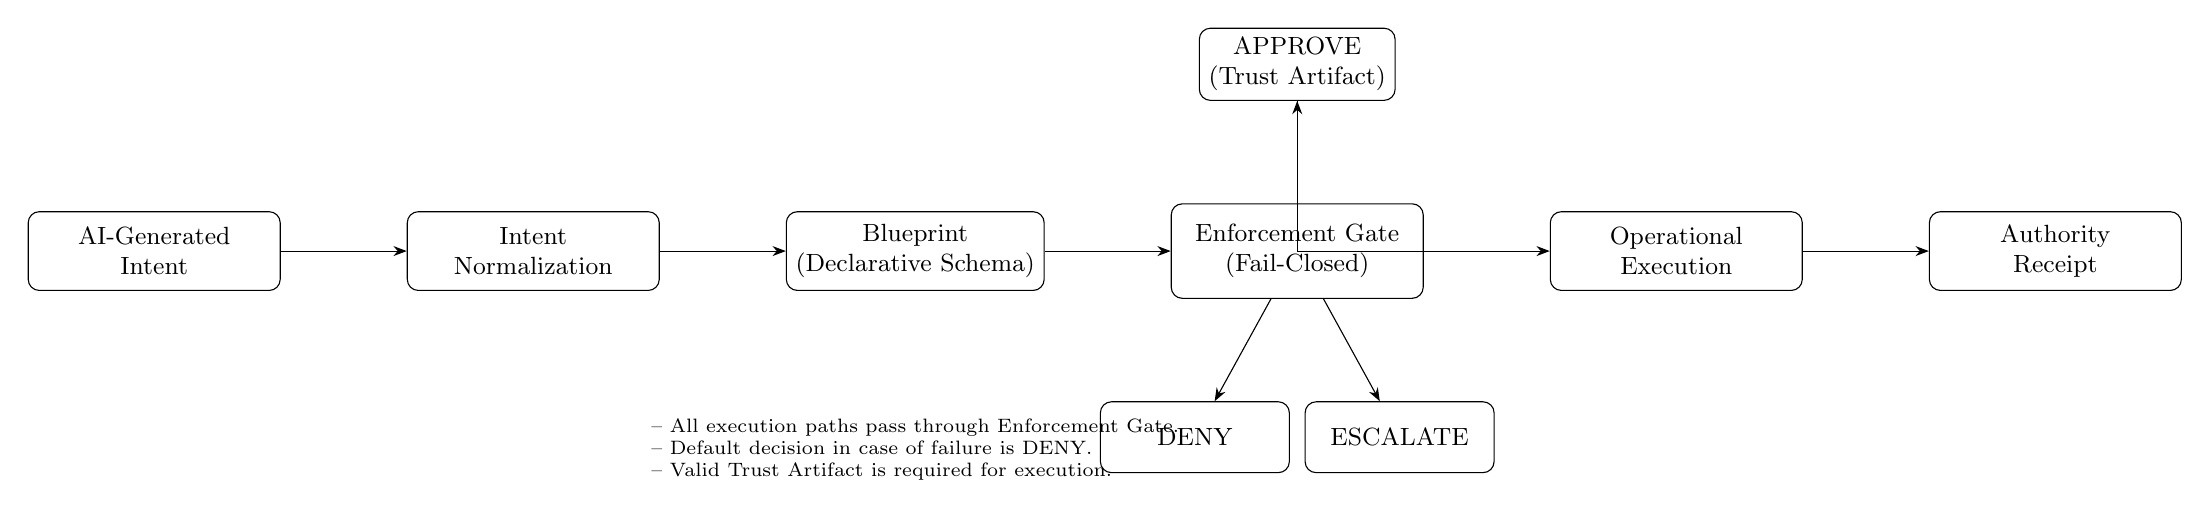
\begin{tikzpicture}[
    node distance=1.8cm and 1.6cm,
    >=Stealth,
    every node/.style={font=\small},
    proc/.style={rectangle, draw, rounded corners, align=center, minimum width=3.2cm, minimum height=1.0cm},
    decision/.style={rectangle, draw, rounded corners, align=center, minimum width=2.4cm, minimum height=0.9cm},
    note/.style={font=\scriptsize}
  ]

  \node[proc] (intent) {AI-Generated\\Intent};
  \node[proc, right=of intent] (norm) {Intent\\Normalization};
  \node[proc, right=of norm] (bp) {Blueprint\\(Declarative Schema)};
  \node[proc, right=of bp, minimum height=1.2cm] (enf) {Enforcement Gate\\(Fail-Closed)};
  \node[proc, right=of enf] (exec) {Operational\\Execution};
  \node[proc, right=of exec] (rcpt) {Authority\\Receipt};

  \draw[->] (intent) -- (norm);
  \draw[->] (norm) -- (bp);
  \draw[->] (bp) -- (enf);
  \draw[->] (exec) -- (rcpt);

  \node[decision, above=1.3cm of enf] (approve) {APPROVE\\(Trust Artifact)};
  \node[decision, below=1.3cm of enf, xshift=-1.3cm] (deny) {DENY};
  \node[decision, below=1.3cm of enf, xshift=1.3cm] (esc) {ESCALATE};

  \draw[->] (enf) -- (approve);
  \draw[->] (enf) -- (deny);
  \draw[->] (enf) -- (esc);
  \draw[->] (approve) |- (exec);

  \node[note, below=1.5cm of bp, align=left] {
    -- All execution paths pass through Enforcement Gate.\\
    -- Default decision in case of failure is DENY.\\
    -- Valid Trust Artifact is required for execution.
  };

  \end{tikzpicture}
  \caption{Deterministic runtime enforcement flow from AI-generated intent through fail-closed authorization to execution and receipt generation.}
  \label{fig:enforcement-flow}
\end{figure}

\subsection{Intent Normalization}

AI operational intent arrives in heterogeneous forms: natural language descriptions, structured API requests, workflow specifications, or combinations thereof. Intent normalization transforms these varied inputs into a canonical intermediate representation suitable for enforcement validation.

\textbf{Input Classes}:

\begin{itemize}
\item \textbf{Natural Language}: ``Schedule follow-up appointment for patient 12345 with Dr. Smith next Tuesday at 2pm''
\item \textbf{Structured API}: \texttt{POST /appointments \{"patient\_id": 12345, "physician\_id": "dr\_smith"\}}
\item \textbf{Workflow Specification}: Declarative YAML/JSON describing multi-step operations with dependencies
\end{itemize}

\textbf{Normalization Process}:

\begin{enumerate}
\item \textbf{Parsing}: Extract syntactic structure from input (NLP parsing for natural language, schema validation for structured inputs)

\item \textbf{Entity Extraction}: Identify operational components:
   \begin{itemize}
   \item \textbf{Operations}: Actions to be performed (create, read, update, delete, invoke, execute)
   \item \textbf{Targets}: Resources operations will affect (databases, APIs, files, external services)
   \item \textbf{Parameters}: Inputs and configuration for operations
   \item \textbf{Dependencies}: Ordering constraints and prerequisites
   \end{itemize}

\item \textbf{Authority Context Extraction}: Determine source identity, authentication method, session context, delegation chain if applicable

\item \textbf{Risk Signal Detection}: Identify factors indicating operational sensitivity (data sensitivity markers, scope modifiers, urgency indicators)
\end{enumerate}

\textbf{Normalized Output}: Structured operation graph with explicit operation nodes, target resources, parameter bindings, and dependency edges. This representation becomes input to Blueprint generation.

\textbf{Determinism Requirement}: Normalization must be deterministic for identical inputs---same intent string produces identical normalized representation. This ensures reproducible enforcement decisions. Probabilistic components (LLM-based parsing) must normalize outputs to deterministic forms.

\subsection{Blueprint Schema}

The Blueprint provides declarative specification of operational intent in machine-verifiable form. The schema encodes all information required for authorization decisions.

\textbf{Core Schema Elements}:

\begin{figure}[t]
  \centering
  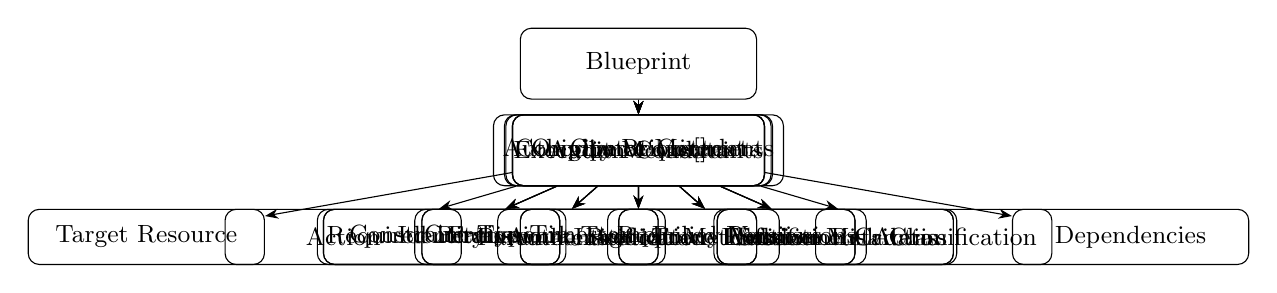
\begin{tikzpicture}[
    level distance=1.1cm,
    sibling distance=2.5cm,
    every node/.style={font=\small},
    root/.style={rectangle, draw, rounded corners, align=center, minimum width=3.0cm, minimum height=0.9cm},
    cat/.style={rectangle, draw, rounded corners, align=center, minimum width=3.2cm, minimum height=0.9cm},
    leaf/.style={rectangle, draw, rounded corners, align=left, minimum width=3.0cm, minimum height=0.7cm},
    edge from parent/.style={draw, ->, >=Stealth}
  ]

  \node[root]{Blueprint}
    child[grow=down]{
      node[cat]{Originator Context}
        child { node[leaf]{Identity} }
        child { node[leaf]{Authentication Method} }
        child { node[leaf]{Session Metadata} }
    }
    child[grow=down]{
      node[cat]{Operations[]}
        child { node[leaf]{Target Resource} }
        child { node[leaf]{Action} }
        child { node[leaf]{Parameters} }
        child { node[leaf]{Required Permissions} }
        child { node[leaf]{Risk Classification} }
        child { node[leaf]{Dependencies} }
    }
    child[grow=down]{
      node[cat]{Authority Requirements}
        child { node[leaf]{Required Permission} }
        child { node[leaf]{Justification} }
        child { node[leaf]{Validation Criteria} }
    }
    child[grow=down]{
      node[cat]{Execution Constraints}
        child { node[leaf]{Constraint Type} }
        child { node[leaf]{Predicate} }
        child { node[leaf]{Enforcement Action} }
    }
    child[grow=down]{
      node[cat]{Compliance Metadata}
        child { node[leaf]{Framework Tags} }
        child { node[leaf]{Policy Versions} }
    }
    child[grow=down]{
      node[cat]{Audit Metadata}
        child { node[leaf]{Creation Timestamp} }
        child { node[leaf]{Trace Identifier} }
    };

  \end{tikzpicture}
  \caption{Declarative Blueprint structure encoding originator context, operations, authority requirements, execution constraints, compliance metadata, and audit metadata.}
  \label{fig:blueprint-structure}
\end{figure}

\begin{lstlisting}[language=Python,caption=Blueprint Core Structure]
Blueprint := {
  blueprint_id: UUID,
  timestamp: DateTime,
  
  originator: {
    identity: Identity,
    authentication_method: AuthMethod,
    session_context: SessionMetadata
  },
  
  operations: Operation[],
  authority_requirements: AuthorityRequirement[],
  execution_constraints: ExecutionConstraint[],
  compliance_metadata: ComplianceTag[],
  audit_metadata: AuditContext
}
\end{lstlisting}

\textbf{Operation Specification}:

\begin{lstlisting}[language=Python,caption=Operation Structure]
Operation := {
  operation_id: UUID,
  target: {
    resource_type: ResourceType,
    resource_id: Identifier,
    namespace: Optional<String>,
    uri: Optional<URI>
  },
  action: ActionType,
  parameters: Parameter[],
  required_permissions: Permission[],
  risk_classification: RiskLevel,
  dependencies: OperationDependency[]
}
\end{lstlisting}

\textbf{Properties}:

\begin{enumerate}
\item \textbf{Declarative}: Blueprints specify \emph{what} will execute, not \emph{how}. Execution details are abstracted.

\item \textbf{Inspectable}: Human-readable structure enables review before execution. Operations, permissions, and constraints are explicit.

\item \textbf{Portable}: Environment-agnostic representation works across cloud, edge, on-premises deployments.

\item \textbf{Immutable}: Once generated, Blueprints cannot be modified. Any change requires new Blueprint with updated identifier.

\item \textbf{Content-Addressable}: Blueprint hash (SHA3-256 of canonical JSON) provides cryptographic identifier binding artifacts to specific Blueprint content.
\end{enumerate}

\subsection{Deterministic Enforcement Gate}

The enforcement gate implements mandatory authorization checkpoint through which all operations must pass before execution.

\textbf{Enforcement Protocol}:

\begin{algorithm}
\caption{Enforcement Protocol}
\label{alg:enforce}
\begin{algorithmic}[1]
\STATE \textbf{function} ENFORCE(blueprint)
\STATE \quad // Stage 1: Structural Validation
\IF{NOT VALIDATE\_SCHEMA(blueprint)}
  \RETURN DENY(``Schema validation failed'')
\ENDIF
\STATE
\STATE \quad // Stage 2: Authority Validation
\STATE \quad authority\_result $\gets$ VALIDATE\_AUTHORITY(blueprint.originator,
\STATE \qquad\qquad\qquad\qquad\qquad blueprint.authority\_requirements)
\IF{authority\_result $\neq$ VALID}
  \RETURN DENY(``Insufficient authority'', authority\_result.gaps)
\ENDIF
\STATE
\STATE \quad // Stage 3: Policy Compliance Validation
\FOR{framework IN blueprint.compliance\_metadata.frameworks}
  \STATE \quad policy\_result $\gets$ EVALUATE\_POLICIES(framework, blueprint)
  \IF{policy\_result $\neq$ COMPLIANT}
    \RETURN DENY(``Policy violation'', framework, policy\_result.violations)
  \ENDIF
\ENDFOR
\STATE
\STATE \quad // Stage 4: Risk Threshold Validation
\IF{blueprint.max\_risk\_level $>$ ACCEPTABLE\_THRESHOLD(blueprint.originator)}
  \RETURN ESCALATE(``Risk threshold exceeded'', blueprint.max\_risk\_level)
\ENDIF
\STATE
\STATE \quad // Stage 5: Dependency Validation
\IF{NOT VALIDATE\_DEPENDENCIES(blueprint.operations)}
  \RETURN DENY(``Dependency validation failed'')
\ENDIF
\STATE
\STATE \quad // Generate Trust Artifact
\STATE \quad artifact $\gets$ GENERATE\_TRUST\_ARTIFACT(blueprint, ``APPROVED'',
\STATE \qquad\qquad\qquad\qquad\qquad\quad validation\_outcomes)
\STATE \quad SIGN(artifact)
\STATE \quad PERSIST\_AUDIT(artifact)
\STATE
\RETURN APPROVE(artifact)
\end{algorithmic}
\end{algorithm}

\textbf{Fail-Closed Semantics}:

\begin{itemize}
\item Default decision is DENY
\item Execution proceeds only upon explicit APPROVE
\item Validation errors, policy conflicts, or system failures result in DENY
\item No ``warn and proceed'' mode---enforcement is mandatory
\end{itemize}

\textbf{Validation Outcomes}:

\begin{itemize}
\item \textbf{APPROVE}: All validation stages passed; Trust Artifact generated with authorization proof
\item \textbf{DENY}: One or more validation stages failed; operation blocked with rationale
\item \textbf{ESCALATE}: Validation conditional on additional authorization (e.g., human review for high-risk operations)
\end{itemize}

\subsection{Trust Artifacts}

Trust Artifacts provide cryptographic evidence of authorization decisions. Each artifact captures complete validation state enabling independent verification.

\begin{figure}[t]
  \centering
  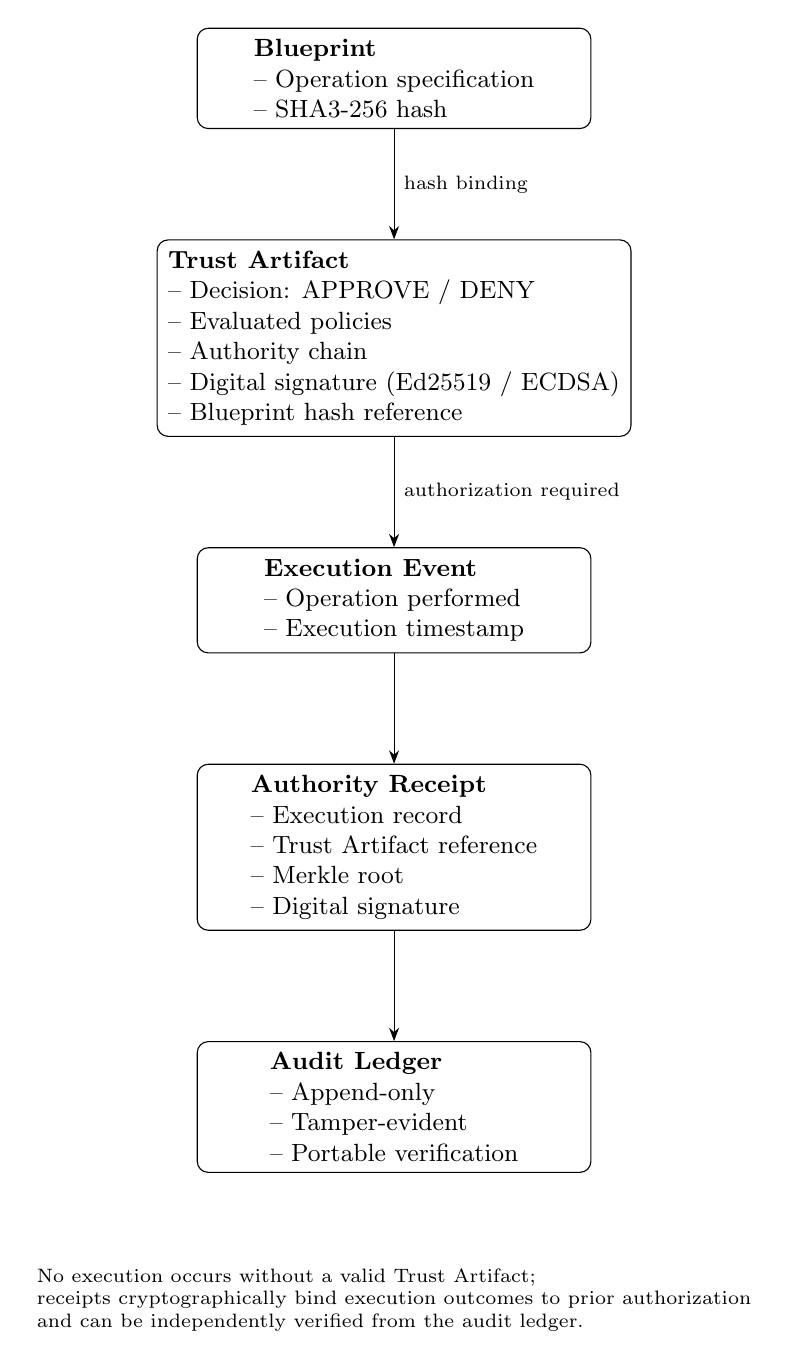
\begin{tikzpicture}[
    node distance=1.4cm,
    >=Stealth,
    every node/.style={font=\small},
    box/.style={rectangle, draw, rounded corners, align=left, minimum width=5.0cm, inner sep=4pt},
    edge label/.style={midway, right, font=\scriptsize}
  ]

  \node[box] (bp) {
    \textbf{Blueprint}\\
    -- Operation specification\\
    -- SHA3-256 hash
  };

  \node[box, below=of bp] (ta) {
    \textbf{Trust Artifact}\\
    -- Decision: APPROVE / DENY\\
    -- Evaluated policies\\
    -- Authority chain\\
    -- Digital signature (Ed25519 / ECDSA)\\
    -- Blueprint hash reference
  };

  \node[box, below=of ta] (exec) {
    \textbf{Execution Event}\\
    -- Operation performed\\
    -- Execution timestamp
  };

  \node[box, below=of exec] (rcpt) {
    \textbf{Authority Receipt}\\
    -- Execution record\\
    -- Trust Artifact reference\\
    -- Merkle root\\
    -- Digital signature
  };

  \node[box, below=of rcpt] (ledger) {
    \textbf{Audit Ledger}\\
    -- Append-only\\
    -- Tamper-evident\\
    -- Portable verification
  };

  \draw[->] (bp) -- node[midway, right, font=\scriptsize]{hash binding} (ta);
  \draw[->] (ta) -- node[midway, right, font=\scriptsize]{authorization required} (exec);
  \draw[->] (exec) -- (rcpt);
  \draw[->] (rcpt) -- (ledger);

  \node[font=\scriptsize, align=left, below=1.1cm of ledger] {
    No execution occurs without a valid Trust Artifact;\\
    receipts cryptographically bind execution outcomes to prior authorization\\
    and can be independently verified from the audit ledger.
  };

  \end{tikzpicture}
  \caption{Cryptographic lineage from Blueprint to Trust Artifact, execution event, Authority Receipt, and append-only audit ledger.}
  \label{fig:artifact-lineage}
\end{figure}

\textbf{Trust Artifact Structure}:

\begin{lstlisting}[language=Python,caption=Trust Artifact Structure]
TrustArtifact := {
  artifact_id: UUID,
  artifact_type: ArtifactType,
  blueprint_hash: SHA3-256,
  timestamp: DateTime,
  
  decision_context: {
    decision: Decision,
    evaluated_policies: PolicyVersionReference[],
    validation_outcomes: ValidationOutcome[],
    decision_rationale: String
  },
  
  authority_chain: AuthorityAssertion[],
  
  signature: {
    algorithm: SignatureAlgorithm,
    public_key_id: KeyID,
    signature_value: Bytes
  },
  
  audit_lineage: {
    parent_artifacts: ArtifactID[],
    trace_id: TraceID
  }
}
\end{lstlisting}

\textbf{Authority Chain}:

\begin{lstlisting}[language=Python,caption=Authority Chain Structure]
AuthorityAssertion := {
  authority_id: Identity,
  assertion_type: AssertionType,  // direct | delegated | system
  delegation_depth: Integer,
  upstream_artifact: Optional<ArtifactID>,
  constraints: DelegationConstraint[]
}
\end{lstlisting}

\textbf{Cryptographic Properties}:

\begin{enumerate}
\item \textbf{Non-Repudiation}: Signature prevents authority from denying authorization decision. Public key cryptography proves artifact originated from enforcement infrastructure.

\item \textbf{Tamper-Evidence}: Any modification to artifact content invalidates signature. Hash binding to Blueprint prevents substitution.

\item \textbf{Verifiable Lineage}: Authority chain references upstream artifacts creating cryptographically verifiable delegation path from root authority to current decision.
\end{enumerate}

\textbf{Signature Generation}:

\begin{lstlisting}[language=Python,caption=Signature Generation]
canonical_json = serialize(artifact, exclude=[signature])
content_hash = SHA3-256(canonical_json)
signature_value = sign(content_hash, private_key)
artifact.signature = {
  algorithm: "Ed25519",
  public_key_id: key_identifier,
  signature_value: signature_value
}
\end{lstlisting}

\subsection{Authority Receipts}

Authority Receipts bind execution outcomes to Trust Artifacts, completing the audit chain from intent through authorization to execution.

\textbf{Authority Receipt Structure}:

\begin{lstlisting}[language=Python,caption=Authority Receipt Structure]
AuthorityReceipt := {
  receipt_id: UUID,
  blueprint_id: UUID,
  trust_artifact_id: UUID,
  execution_timestamp: DateTime,
  
  execution_records: ExecutionRecord[],
  
  compliance_attestation: {
    frameworks: FrameworkID[],
    attestation_claims: Claim[],
    evidence_references: AuditEntryID[]
  },
  
  portable_proof: {
    merkle_root: Hash,
    merkle_proof: MerkleProof,
    verifier_instructions: VerificationProtocol
  },
  
  signature: Signature
}
\end{lstlisting}

\textbf{Portable Proof Construction}:

Authority Receipts include Merkle proofs enabling verification without access to complete audit infrastructure. This enables external auditors to verify that:
\begin{enumerate}
\item Receipt is authentic (signature verification)
\item Receipt is included in authorized artifact chain (Merkle proof)
\item Blueprint was authorized (trust artifact verification)
\item Execution matched authorized Blueprint (operation IDs align)
\end{enumerate}

\section{Formal Properties}
\label{sec:properties}

This section analyzes formal properties of the enforcement model with explicit acknowledgment of limitations.

\subsection{Determinism}

\paragraph{Property P1 (Deterministic Validation)} Given identical Blueprint and policy framework versions, enforcement validation produces identical authorization decisions.

\textbf{Formalization}:

\begin{equation}
\forall b, p, s_1, s_2: (s_1.policies = p \land s_2.policies = p) \implies \text{enforce}(b, s_1) = \text{enforce}(b, s_2)
\end{equation}

\textbf{Proof Sketch}: Enforcement validation (Section~\ref{sec:model}) consists of deterministic operations: schema validation (structural checks), authority validation (permission set comparison), policy evaluation (predicate evaluation over Blueprint), and risk threshold comparison. Given identical inputs (Blueprint, policies), these operations produce identical outputs.

\textbf{Limitation}: Determinism assumes stable policy framework versions. Policy updates between validation invocations may produce different results for identical Blueprints, which is intended behavior. Determinism also assumes bug-free implementation of validation logic.

\subsection{Non-Bypassability}

\paragraph{Property P2 (Non-Bypassability)} Under trust assumptions TA1-TA4, AI systems cannot execute operations without passing through enforcement gate.

\textbf{Formalization}:

\begin{equation}
\begin{split}
\forall o: \text{executed}(o) \implies & \\
\exists b, a: & (b.\text{operations contains } o) \land \\
& (a.\text{blueprint\_hash} = \text{hash}(b)) \land \\
& (a.\text{decision} = \text{APPROVE}) \land \\
& \text{verify\_trust\_artifact}(a) = \text{VALID}
\end{split}
\end{equation}

\textbf{Architectural Requirement}: Enforcement layer must be positioned such that execution infrastructure accepts only Blueprints accompanied by valid Trust Artifacts. This requires:

\begin{enumerate}
\item Execution APIs modified to require Trust Artifact presentation
\item Network topology prevents direct access to execution infrastructure bypassing enforcement
\item Enforcement infrastructure operates with higher privilege than AI systems
\end{enumerate}

\textbf{Limitation}: Non-bypassability is architectural property dependent on correct deployment. If execution infrastructure is misconfigured to accept operations without Trust Artifacts, the property does not hold. The model prevents logical bypass (AI systems cannot forge valid Trust Artifacts) but cannot prevent deployment errors.

\subsection{Pre-Execution Constraint Validation}

\paragraph{Property P3 (Pre-Execution Validation)} Authorization decisions occur strictly before execution.

\textbf{Formalization}:

\begin{equation}
\forall o, a, r: (a \text{ authorizes } o) \land (r \text{ documents execution of } o) \implies a.\text{timestamp} < r.\text{execution\_timestamp}
\end{equation}

\textbf{Enforcement Protocol Guarantee}: The enforcement protocol generates Trust Artifacts before returning APPROVE decision. Execution infrastructure accepts only approved Blueprints with Trust Artifacts. Therefore, temporal ordering is structurally guaranteed.

\textbf{Limitation}: Execution infrastructure must respect Trust Artifact validity windows. If significant time elapses between authorization and execution, policies may have changed or delegated authority may have expired. Implementations should validate authority chain freshness at execution time.

\subsection{Audit Completeness}

\paragraph{Property P4 (Audit Completeness)} Every execution has corresponding audit trail from intent through authorization to outcome.

\textbf{Formalization}:

\begin{equation}
\begin{split}
\forall o: \text{executed}(o) \implies & \\
\exists b, a, r: & (b.\text{operations contains } o) \land \\
& (a.\text{blueprint\_hash} = \text{hash}(b)) \land \\
& (r.\text{blueprint\_id} = b.\text{blueprint\_id}) \land \\
& (r.\text{trust\_artifact\_id} = a.\text{artifact\_id}) \land \\
& \text{audit\_ledger contains } \{b, a, r\}
\end{split}
\end{equation}

\textbf{Protocol Guarantee}: Enforcement protocol appends Trust Artifacts to audit ledger before approving execution. Receipt generation protocol appends Authority Receipts after execution completion. Both operations are mandatory.

\textbf{Limitation}: Completeness depends on audit ledger availability. If ledger append fails, enforcement protocol must deny execution (fail-closed). However, between successful execution and receipt generation, a window exists where operation executed but receipt not yet persisted. Implementations should handle receipt generation failures through retry mechanisms.

\subsection{Lineage Integrity}

\paragraph{Property P5 (Lineage Integrity)} Authority chains in Trust Artifacts form valid directed acyclic graphs from root authorities to current assertions.

\textbf{Formalization}:

\begin{equation}
\begin{split}
\forall a, \text{auth} \in a.\text{authority\_chain}: & \\
\text{auth}.\text{assertion\_type} = \text{``delegated''} \implies & \\
\exists u \in \text{audit\_ledger}: & (u.\text{artifact\_id} = \text{auth}.\text{upstream\_artifact}) \land \\
& (u.\text{timestamp} < a.\text{timestamp}) \land \\
& \text{verify\_trust\_artifact}(u) = \text{VALID} \land \\
& \neg \text{creates\_cycle}(a, u)
\end{split}
\end{equation}

\textbf{Validation Enforcement}: Authority chain validation recursively verifies upstream artifacts ensuring:
\begin{enumerate}
\item Upstream artifacts exist and are valid
\item Temporal ordering is consistent (upstream precedes downstream)
\item Delegation constraints are satisfied
\item No cycles exist in delegation graph
\end{enumerate}

\textbf{Limitation}: The model verifies that delegation chains are structurally valid but cannot verify that root authorities should possess their claimed authority. If a root authority is compromised or malicious, derived delegations will be structurally valid despite originating from untrustworthy source.

\subsection{Properties Summary}

\begin{table}[htbp]
\centering
\caption{Formal Properties Summary}
\label{tab:properties}
\begin{tabular}{@{}lll@{}}
\toprule
\textbf{Property} & \textbf{Guarantee} & \textbf{Limitation} \\
\midrule
P1: Determinism & Identical inputs $\rightarrow$ identical decisions & Stable policies, bug-free code \\
P2: Non-Bypassability & Operations require valid authorization & Correct deployment \\
P3: Pre-Execution & Authorization precedes execution & Validity windows \\
P4: Audit Completeness & Every execution has audit trail & Ledger availability \\
P5: Lineage Integrity & Valid delegation chains & Root authority trust \\
\bottomrule
\end{tabular}
\end{table}

\section{Comparative Analysis}
\label{sec:comparison}

This section compares the enforcement model against alternative governance approaches.

\subsection{Process-Based Governance}

\textbf{Approach}: Organizations document governance policies, train personnel, implement organizational controls, and audit compliance through periodic reviews.

\textbf{Examples}: ISO 42001 management systems, organizational AI ethics committees, documented approval workflows.

\textbf{Structural Difference}: Process-based governance assumes organizational discipline. The enforcement model provides architectural constraint.

\begin{table}[htbp]
\centering
\caption{Process-Based vs Enforcement Model Comparison}
\label{tab:process_comparison}
\begin{tabular}{@{}lll@{}}
\toprule
\textbf{Dimension} & \textbf{Process-Based} & \textbf{Enforcement Model} \\
\midrule
Compliance Verification & Trust-based & Cryptographic \\
Enforcement Timing & Post-execution & Pre-execution \\
Bypass Resistance & Weak & Strong \\
Audit Evidence & Mutable logs & Tamper-evident \\
Operational Overhead & Documentation & Validation latency \\
\bottomrule
\end{tabular}
\end{table}

\textbf{Complementarity}: The enforcement model does not replace organizational governance. Policy frameworks must be specified through organizational processes. The model enforces specified policies rather than determining what policies should exist.

\subsection{Risk-Tier Governance}

\textbf{Approach}: Systems classified by risk level with oversight requirements scaled accordingly.

\textbf{Examples}: EU AI Act risk tiers, NIST AI RMF risk categorization.

\textbf{Structural Difference}: Risk-tier governance classifies systems at deployment time. The enforcement model classifies operations at execution time.

\begin{table}[htbp]
\centering
\caption{Risk-Tier vs Enforcement Model Comparison}
\label{tab:risk_comparison}
\begin{tabular}{@{}lll@{}}
\toprule
\textbf{Dimension} & \textbf{Risk-Tier} & \textbf{Enforcement Model} \\
\midrule
Classification Granularity & System-level & Operation-level \\
Classification Timing & Deployment (static) & Execution (dynamic) \\
Context Sensitivity & Low & High \\
Compliance Burden & Uniform per tier & Scaled to risk \\
\bottomrule
\end{tabular}
\end{table}

\textbf{Integration}: The enforcement model can implement risk-tier requirements. High-risk operations trigger enhanced validation (e.g., mandatory human review) while low-risk operations proceed with lightweight validation.

\subsection{Logging-Only Systems}

\textbf{Approach}: AI systems execute operations freely while generating comprehensive logs for post-execution analysis.

\textbf{Structural Difference}: Logging detects violations after execution. The enforcement model prevents violations before execution.

\textbf{Complementarity}: The enforcement model generates audit logs as byproduct of enforcement (Trust Artifacts, Authority Receipts). Logging provides forensic value even with enforcement.

\subsection{Post-Hoc Audit Models}

\textbf{Approach}: Periodic audits review AI system behavior through sampling outputs, testing scenarios, and interviewing operators.

\textbf{Structural Difference}: Post-hoc audits examine historical behavior. The enforcement model constrains future behavior.

\textbf{Complementarity}: Post-hoc audits can verify enforcement effectiveness. Auditors sample Trust Artifacts and verify they demonstrate appropriate authorization decisions.

\subsection{Comparative Summary}

The enforcement model provides complementary capabilities to existing approaches:

\begin{itemize}
\item \textbf{Process governance} defines policies; enforcement ensures policies constrain operations
\item \textbf{Risk classification} determines oversight rigor; enforcement implements oversight mechanisms
\item \textbf{Logging} provides forensic evidence; enforcement prevents violations requiring forensics
\item \textbf{Audits} verify governance effectiveness; enforcement provides verifiable evidence for audits
\end{itemize}

Integration with existing frameworks strengthens overall governance posture by adding deterministic constraint to process-based foundations.

\section{Implementation Considerations}
\label{sec:implementation}

A reference implementation demonstrates the model's feasibility. This section discusses implementation challenges and design choices.

\subsection{Latency and Throughput}

\textbf{Challenge}: Enforcement validation introduces latency between intent submission and execution completion.

\textbf{Latency Sources}:
\begin{enumerate}
\item Blueprint generation: Intent parsing and normalization (10-100ms)
\item Policy evaluation: Validation against governance frameworks (5-50ms)
\item Cryptographic operations: Signature generation and verification (1-10ms)
\item Audit persistence: Ledger append operations (10-100ms)
\end{enumerate}

\textbf{Total Latency}: 25-250ms depending on Blueprint complexity and policy framework count.

\textbf{Mitigation Strategies}:

\begin{itemize}
\item \textbf{Caching}: Policy evaluation results cached keyed by (Blueprint hash, policy version). Cache hit eliminates policy evaluation latency.
\item \textbf{Parallel Validation}: Multiple policy frameworks evaluated concurrently.
\item \textbf{Asynchronous Audit}: Trust Artifact persistence occurs asynchronously after APPROVE decision with retry mechanisms for failures.
\item \textbf{Tiered Enforcement}: Low-risk operations use lightweight validation; high-risk operations justify comprehensive validation latency.
\end{itemize}

\textbf{Throughput}: Reference implementation achieves 1,000-5,000 enforcements/second on commodity hardware depending on Blueprint complexity. Horizontal scaling via stateless enforcement nodes supports higher throughput.

\subsection{Deployment Boundaries}

\textbf{Enforcement Placement}:

The model requires positioning enforcement layer between AI systems and execution infrastructure. Three deployment patterns emerge:

\textbf{Pattern A: Centralized Gateway}
\begin{itemize}
\item Enforcement layer deployed as API gateway
\item All execution requests route through gateway
\item Advantages: Centralized policy management, uniform audit collection
\item Disadvantages: Single point of failure, network latency
\end{itemize}

\textbf{Pattern B: Embedded Enforcement}
\begin{itemize}
\item Enforcement layer embedded within AI system process
\item Trust Artifacts generated locally
\item Advantages: Low latency, continues during network partitions
\item Disadvantages: Distributed policy synchronization, enforcement tampering risk
\end{itemize}

\textbf{Pattern C: Sidecar Enforcement}
\begin{itemize}
\item Enforcement layer deployed as sidecar container alongside AI systems
\item Kubernetes or service mesh integration
\item Advantages: Isolation from AI system, infrastructure-level guarantees
\item Disadvantages: Container orchestration dependency
\end{itemize}

The reference implementation supports all three patterns through adapter interfaces.

\subsection{Edge vs Cloud Considerations}

\textbf{Edge Deployment}:

Edge environments (IoT devices, autonomous vehicles, field equipment) present unique challenges:

\begin{itemize}
\item \textbf{Limited Resources}: Edge devices may lack computational capacity for complex policy evaluation
\item \textbf{Intermittent Connectivity}: Cannot rely on cloud-based enforcement during offline periods
\item \textbf{Local Policy Caching}: Must cache policies locally with periodic synchronization
\item \textbf{Audit Queuing}: Audit artifacts queue locally and upload when connectivity available
\end{itemize}

\textbf{Strategy}: Tiered enforcement where edge performs lightweight validation (authority chain verification, basic permission checks) with critical operations deferred to cloud enforcement when connectivity permits.

\textbf{Cloud Deployment}:

Cloud environments provide:
\begin{itemize}
\item \textbf{Elastic Scaling}: Enforcement infrastructure scales with demand
\item \textbf{Centralized Audit}: Unified audit ledger across distributed operations
\item \textbf{Policy Consistency}: Single policy source propagated to enforcement nodes
\item \textbf{High Availability}: Redundant enforcement nodes with load balancing
\end{itemize}

\textbf{Hybrid Approach}: Low-risk operations validated at edge for latency; high-risk operations escalate to cloud for comprehensive validation.

\subsection{Multi-Tenant Considerations}

\textbf{Challenge}: Multiple organizations sharing enforcement infrastructure require tenant isolation.

\textbf{Requirements}:
\begin{enumerate}
\item \textbf{Policy Isolation}: Tenant A's policies do not affect Tenant B's enforcement
\item \textbf{Audit Isolation}: Tenants cannot access each other's audit artifacts
\item \textbf{Cryptographic Isolation}: Separate signing keys per tenant
\item \textbf{Resource Isolation}: Tenant A's load does not impact Tenant B's latency
\end{enumerate}

\textbf{Implementation Strategies}:

\begin{itemize}
\item \textbf{Logical Isolation}: Single enforcement infrastructure with tenant-scoped policies and audit partitioning
\item \textbf{Physical Isolation}: Dedicated enforcement instances per tenant
\item \textbf{Hybrid}: Shared infrastructure for non-sensitive validation with tenant-specific signing and audit
\end{itemize}

The reference implementation uses logical isolation with cryptographic tenant ID binding in Trust Artifacts preventing cross-tenant artifact acceptance.

\subsection{Policy Update Mechanisms}

\textbf{Challenge}: Policies evolve over time. Enforcement must handle policy updates without disrupting operations.

\textbf{Update Protocol}:
\begin{enumerate}
\item New policy version published to policy registry
\item Enforcement nodes receive update notification
\item Nodes fetch new policy version
\item Nodes maintain both old and new versions during transition period
\item New Blueprints validated against new policy version
\item In-flight operations validated against policy version active at Blueprint generation time
\end{enumerate}

\textbf{Versioning}:
Trust Artifacts reference specific policy versions enabling reproducible compliance verification. Historical artifacts remain valid under historical policies.

\textbf{Rollback}:
If policy update causes unexpected denials, administrators can rollback to previous version. Rollback does not invalidate Trust Artifacts generated under new version---they remain valid as historical artifacts.

\subsection{Evaluation Scope}

This work presents an architectural and formal model. Empirical benchmarking and large-scale deployment evaluation remain future work.

\section{Limitations}
\label{sec:limitations}

\subsection{Model Limitations}

\textbf{L1. Intent Generation Layer}: The model constrains execution but does not prevent AI systems from generating malicious intent. Adversarial prompts, model poisoning, or emergent capabilities may cause AI systems to propose unauthorized operations. The model blocks execution but cannot prevent intent generation.

\textbf{L2. Root Authority Verification}: The model verifies that authority chains are structurally valid (proper delegation, signature verification) but cannot verify that root authorities should possess claimed permissions. Compromised or malicious root authorities can authorize harmful operations while maintaining procedural compliance.

\textbf{L3. Policy Specification Burden}: Effectiveness depends on comprehensive policy specification. Incomplete policies create enforcement gaps permitting non-compliant operations. The model enforces declared policies but does not guarantee the completeness or correctness of those policies.

\textbf{L4. Semantic vs Syntactic Compliance}: The model enforces syntactic policy compliance (operations possess required permissions, constraints satisfied) but cannot verify semantic compliance (operations achieve intended outcomes). Sophisticated adversaries may craft operations satisfying policies syntactically while achieving harmful outcomes semantically.

\subsection{Implementation Limitations}

\textbf{L5. Deployment Correctness}: Non-bypassability (Property P2) requires correct architectural deployment. Misconfigured execution infrastructure accepting operations without Trust Artifacts negates enforcement. The model provides enforcement mechanism but correct deployment remains implementation responsibility.

\textbf{L6. Enforcement Layer Integrity}: The model assumes enforcement infrastructure operates correctly (Trust Assumption TA1). Compromised enforcement infrastructure can issue fraudulent Trust Artifacts authorizing unauthorized operations. Hardware security modules or trusted execution environments can strengthen this assumption but add deployment complexity.

\textbf{L7. Audit Ledger Availability}: Audit completeness (Property P4) depends on ledger availability. If audit persistence fails, enforcement must deny operations (fail-closed). This prioritizes security over availability, which may be inappropriate for availability-critical applications.

\textbf{L8. Validation Latency}: Enforcement validation introduces latency. For latency-critical applications (real-time control systems, high-frequency trading), validation overhead may exceed acceptable bounds. Implementations must balance security and performance.

\subsection{Organizational Limitations}

\textbf{L9. Human Authority Fallibility}: The model provides verifiable record of authorization decisions but cannot prevent poor human judgment. If authorized humans approve harmful operations, those operations execute with valid Trust Artifacts. The model enables accountability through cryptographic non-repudiation but does not replace sound human decision-making.

\textbf{L10. Not a Complete Governance Solution}: The model addresses execution control but does not replace comprehensive AI governance including model development standards, data governance, transparency requirements, and incident response. It provides technical substrate for governance rather than complete governance framework.

\textbf{L11. Organizational Change Requirement}: Adoption requires organizational process changes: AI systems must submit intents through enforcement layer rather than directly invoking execution APIs. Policies must be formalized in declarative specifications. Operations staff must monitor enforcement infrastructure. Organizations resistant to process change may find adoption challenging.

\subsection{Acknowledgment}

These limitations do not invalidate the model but establish realistic expectations. The model enables governance through architectural constraint within acknowledged boundaries. Future work should address limitations through:

\begin{itemize}
\item Intent generation constraints complementing execution constraints
\item Enhanced root authority verification through multi-party authorization
\item Automated policy completeness analysis
\item Semantic policy verification techniques
\item Deployment validation tooling
\item Enforcement infrastructure hardening
\item Latency optimization for critical applications
\end{itemize}

\section{Conclusion}
\label{sec:conclusion}

This paper has presented a deterministic runtime enforcement model for AI governance positioning mandatory authorization checkpoints at the operational boundary where AI-generated intent transitions to system execution. The model employs Blueprint intermediate schema to declaratively encode operational intent with explicit authority requirements, risk classifications, and execution constraints. Enforcement occurs through cryptographic Trust Artifacts providing verifiable evidence of pre-execution authorization decisions with fail-closed semantics preventing unauthorized operations.

Analysis demonstrates that the model provides formal properties including deterministic validation, non-bypassability under stated assumptions, pre-execution constraint validation, audit completeness, and lineage integrity. Comparative analysis shows the model provides complementary capabilities to existing process-based governance frameworks by adding deterministic constraint to organizational governance foundations.

A reference implementation validates the model's feasibility with latency analysis demonstrating 25-250ms enforcement overhead and throughput supporting 1,000-5,000 enforcements/second on commodity hardware. Implementation considerations address deployment patterns, edge versus cloud tradeoffs, multi-tenant isolation, and policy update mechanisms.

Acknowledged limitations include inability to prevent malicious intent generation, dependence on comprehensive policy specification, deployment correctness requirements, and organizational change burden. These limitations establish realistic expectations while demonstrating that the model enables governance through architectural constraint within acknowledged boundaries.

\subsection{Contributions}

This work formalizes execution-bound governance as an architectural layer with cryptographic enforcement properties. The Blueprint schema, Trust Artifact structure, and enforcement protocol provide formal specifications for deterministic authorization validation.

\subsection{Future Work}

Several directions merit investigation:

\textbf{Empirical Evaluation}: Large-scale deployment studies measuring enforcement overhead in production environments, analyzing denial patterns revealing attempted policy violations, and evaluating policy specification burden across domains.

\textbf{Standardization}: Development of standard Blueprint schema formats enabling cross-implementation interoperability, policy specification language standards, and Trust Artifact verification protocols supporting portable compliance verification.

\textbf{Enhanced Properties}: Exploring privacy-preserving verification through zero-knowledge proofs enabling compliance verification without revealing operational details, quantum-resistant cryptography for long-term audit integrity, and Byzantine fault tolerant enforcement supporting adversarial environments.

\textbf{Integration Research}: Investigating integration with existing AI governance frameworks, mapping Blueprint enforcement to regulatory compliance requirements, and developing automated policy synthesis from regulatory texts.

\textbf{Formal Verification}: Applying formal methods to verify enforcement protocol correctness, proving security properties under cryptographic assumptions, and model checking for enforcement bypass vulnerabilities.

The governance verification gap represents a fundamental challenge as AI systems transition to operational infrastructure. The enforcement model presented here demonstrates that architectural solutions can provide verifiable constraint where process-based approaches fall short. This work formalizes execution-bound governance and demonstrates its enforceability under defined assumptions.

\bibliographystyle{plain}
\bibliography{references}

\appendix

\section{Blueprint Schema Example}

\begin{lstlisting}[language=json,caption=Sample Blueprint Instance]
{
  "blueprint_id": "550e8400-e29b-41d4-a716-446655440000",
  "timestamp": "2026-02-07T14:30:00Z",
  
  "originator": {
    "identity": "user@example.com",
    "authentication_method": "multi_factor",
    "session_context": {
      "session_id": "sess_abc123",
      "source_ip": "192.0.2.1"
    }
  },
  
  "operations": [
    {
      "operation_id": "660e8400-e29b-41d4-a716-446655440001",
      "target": {
        "resource_type": "database",
        "resource_id": "customer_records",
        "namespace": "production"
      },
      "action": "write",
      "parameters": [
        {
          "name": "table",
          "value": "customers",
          "type": "string",
          "sensitivity": "internal"
        }
      ],
      "required_permissions": [
        {
          "scope": "database_service",
          "action": "write",
          "resource_pattern": "customer_records.*"
        }
      ],
      "risk_classification": "medium",
      "dependencies": []
    }
  ],
  
  "authority_requirements": [
    {
      "required_permission": {
        "scope": "database_service",
        "action": "write",
        "resource_pattern": "customer_records.*"
      },
      "justification": "GDPR Article 5(1)(f)",
      "validation_criteria": []
    }
  ],
  
  "compliance_metadata": {
    "frameworks": ["gdpr", "iso_42001"]
  }
}
\end{lstlisting}

\end{document}
